% pdflatex map_sheet.tex
% TODO: add this to the Makefile.
\documentclass[parskip]{scrartcl}
\usepackage{graphicx,overpic}
% Consider making margins either 0 or 0.1in.
\usepackage[paperheight=17in,paperwidth=11in,margin=0.25in]{geometry}

\usepackage{geometry}
\usepackage{multicol}
\usepackage{amsmath}
\usepackage{titlesec}
\usepackage{diagbox,pict2e}
\usepackage{makecell}
\usepackage{tabularx}
\usepackage{multirow}
\usepackage{lscape}
\usepackage{tikz}
\usepackage{adjustbox}


\begin{document}

\begin{center}
  \begin{overpic}[width=10.5in, grid=false]{map.pdf}

    \put(-60, 10){\includegraphics[angle=-90,width=11in]{../rules/nv-air-status.pdf}}

    % Victory Points Track (PDF from ../rules/)
    % \put(-20, 85){\includegraphics[width=5in]{../rules/victory-points.pdf}}

    % US side
    \put(50, -60){\rotatebox{90}{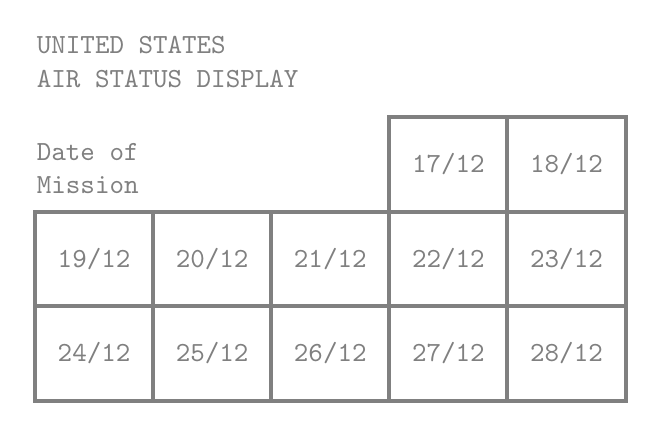
\begin{tikzpicture}
    \newcommand{\lw}{0.5mm}
    \tikzset{lwstyle/.style={line width=\lw}}
    \definecolor{svggray}{RGB}{128,128,128}
    \tikzset{every node/.style={text=svggray}, every path/.style={draw=svggray}}


    \node[anchor=west, align=left] at (-0.1, 0.7) {%
        \ttfamily\textbf{UNITED STATES} \\
        \ttfamily \textbf{AIR STATUS DISPLAY}%
    };

    \node[anchor=west, align=left] at (-0.1, -0.65) {%
        \ttfamily\textbf{Date of} \\
        \ttfamily\textbf{Mission}%
    };

    % Define box size
    \def\boxwidth{1.5}
    \def\boxheight{1.2}

    \foreach \x [count=\i] in {17, 18} {
        \pgfmathsetmacro\xpos{\i + 2}
        \draw[lwstyle] (\xpos*\boxwidth, 0) rectangle (\xpos*\boxwidth + \boxwidth, -\boxheight);
        \node at (\xpos*\boxwidth + 0.75, -0.6) {\ttfamily \textbf{\x/12}};
    }

    % Second row (middle row)
    \foreach \x [count=\i] in {19, 20, 21, 22, 23} {
        \pgfmathsetmacro\xpos{\i - 1}
        \draw[lwstyle] (\xpos*\boxwidth, -\boxheight) rectangle (\xpos*\boxwidth + \boxwidth, -2*\boxheight);
        \node at (\xpos*\boxwidth + 0.75, -1.8) {\ttfamily \textbf{\x/12}};
    }

    % Third row (bottom row)
    \foreach \x [count=\i] in {24, 25, 26, 27, 28} {
        \pgfmathsetmacro\xpos{\i - 1}
        \draw[lwstyle] (\xpos*\boxwidth, -2*\boxheight) rectangle (\xpos*\boxwidth + \boxwidth, -3*\boxheight);
        \node at (\xpos*\boxwidth + 0.75, -3.0) {\ttfamily \textbf{\x/12}};
    }
\end{tikzpicture}
}}
    \put(50, -30){\rotatebox{90}{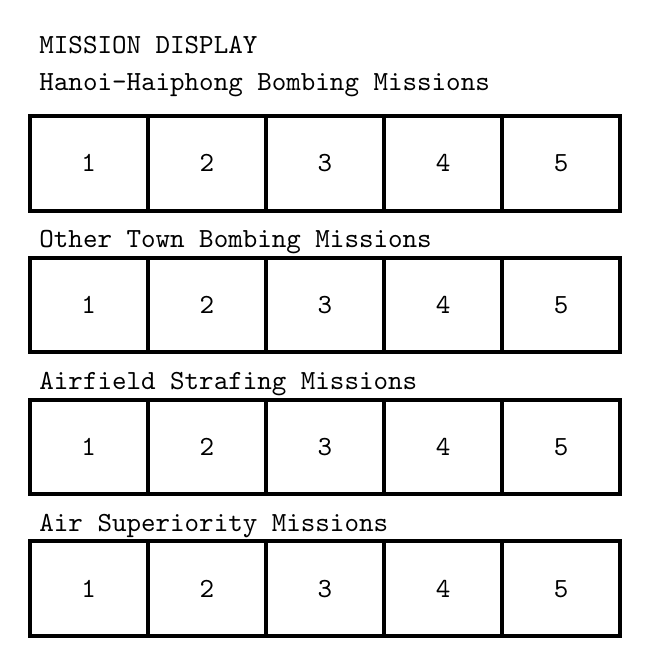
\begin{tikzpicture}
    % Define box size
    \def\boxwidth{1.5}
    \def\boxheight{1.2}
    \def\spacing{0.5} % Space between text and boxes
    \newcommand{\lw}{0.5mm}
    \tikzset{lwstyle/.style={line width=\lw}}

    \node[anchor=west, align=left] at (0.0, 0.9) {%
        \ttfamily\textbf{MISSION DISPLAY}
    };



    % Categories
    \node[anchor=west] at (0.0, 0.4) {\ttfamily \textbf{Hanoi-Haiphong Bombing Missions}};
    \node[anchor=west] at (0.0, -1.6) {\ttfamily \textbf{Other Town Bombing Missions}};
    \node[anchor=west] at (0.0, -3.4) {\ttfamily \textbf{Airfield Strafing Missions}};
    \node[anchor=west] at (0.0, -5.2) {\ttfamily \textbf{Air Superiority Missions}};

    % Draw the boxes for each category
    \foreach \y in {0, -1.8, -3.6, -5.4} {
        \foreach \x in {0,1,2,3,4} {
            \draw[lwstyle] (\x*\boxwidth, \y) rectangle (\x*\boxwidth + \boxwidth, \y-\boxheight);
            \node at (\x*\boxwidth + 0.75, \y-0.6) {\ttfamily \textbf{\the\numexpr\x+1}};
        }
    }
\end{tikzpicture}
}}


    \put(5, -65){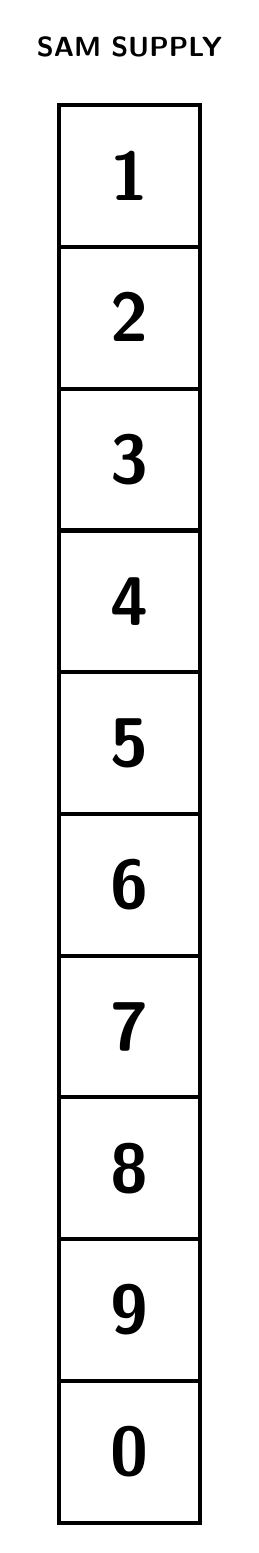
\begin{tikzpicture}
    % Define box properties
    \def\boxwidth{1.8}
    \def\boxheight{1.8}
    \def\boxthickness{1.5pt} % Adjustable line thickness

    % Define SAM Supply numbers (1 to 0)
    \def\samsupply{1, 2, 3, 4, 5, 6, 7, 8, 9, 0}

    % Title at the top
    \node[anchor=south] at (0.9, 0.5) {\sffamily \bfseries SAM SUPPLY};

    % Draw boxes and numbers
    \foreach \x [count=\i] in \samsupply {
        \pgfmathsetmacro\ypos{-(\i-1) * \boxheight} % Calculate vertical position
        \draw[line width=\boxthickness] (0, \ypos) rectangle (\boxwidth, \ypos - \boxheight);
        \node at (0.9, \ypos - 0.9) {\sffamily \bfseries \Huge \x}; % Centered inside box
    }

\end{tikzpicture}
}
    \put(90, -55){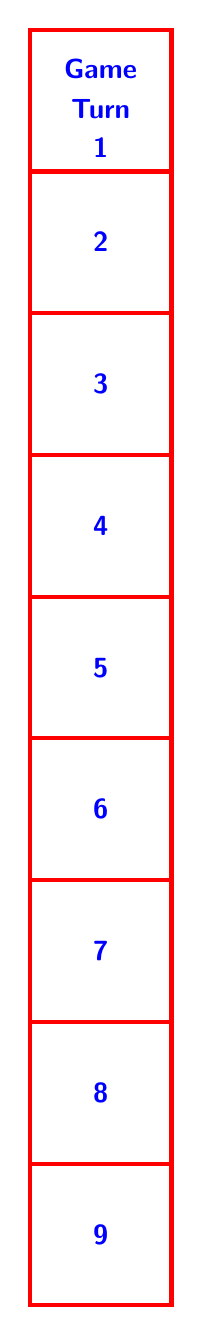
\begin{tikzpicture}

  % Define the gray color matching SVG default gray
  \definecolor{svggray}{RGB}{128,128,128}
  
  % Apply to everything
  \tikzset{every picture/.style={color=red}}

  \tikzset{every node/.style={text=blue}, every path/.style={draw=red}}


    % Define box properties
    \def\boxwidth{1.8}
    \def\boxheight{1.8}
    \def\boxthickness{1.5pt} % Adjustable line thickness

    % Define Game Turn numbers (2 to 9, since 1 is in the title box)
    \def\gameturns{2, 3, 4, 5, 6, 7, 8, 9}

    % First box with "Game Turn 1"
    \draw[line width=\boxthickness] (0, 0) rectangle (\boxwidth, -\boxheight);
    \node at (0.9, -0.5) {\sffamily \bfseries Game};
    \node at (0.9, -1.0) {\sffamily \bfseries Turn};
    \node at (0.9, -1.5) {\sffamily \bfseries 1};

    % Draw boxes and numbers for turns 2-9
    \foreach \x [count=\i] in \gameturns {
        \pgfmathsetmacro\ypos{-\i * \boxheight} % Calculate vertical position
        \draw[line width=\boxthickness] (0, \ypos) rectangle (\boxwidth, \ypos - \boxheight);
        \node at (0.9, \ypos - 0.9) {\sffamily \bfseries \x}; % Centered inside box
    }
\end{tikzpicture}
}
    \put(10, -75){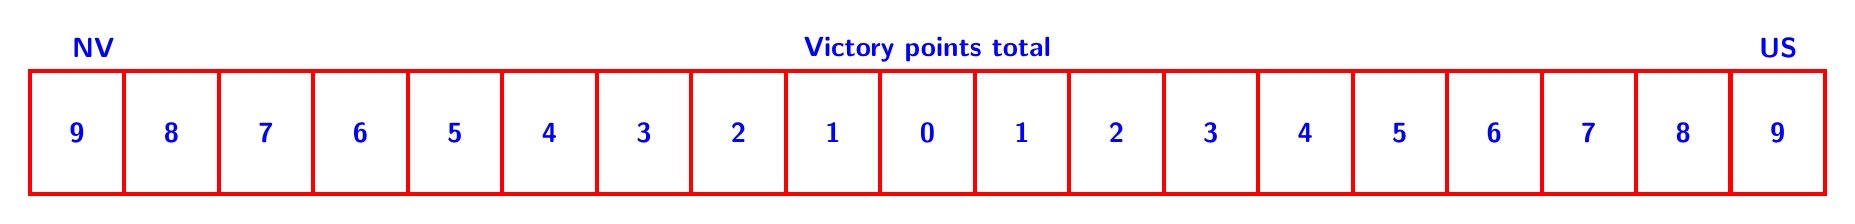
\begin{tikzpicture}[scale=1.2]
    \tikzset{every node/.style={text=blue}, every path/.style={draw=red}}

    % Define box size
    \def\boxwidth{1.0}
    \def\boxheight{1.3}
    \def\boxthickness{1.5pt} % Parameterized line thickness

    % Define victory points (NV decreasing, US increasing)
    \def\victorypoints{9, 8, 7, 6, 5, 4, 3, 2, 1, 0, 1, 2, 3, 4, 5, 6, 7, 8, 9}

    \def\ypos{0.25}
    % Labels
    \node[anchor=east] at (1, \ypos) {\sffamily \bfseries NV};
    \node[anchor=west] at (18*\boxwidth + 0.2, \ypos) {\sffamily \bfseries US};
    \node[anchor=south] at (9.5*\boxwidth, \ypos-0.25) {\sffamily \bfseries Victory points total}; % Centered over the track

    % Draw boxes and numbers
    \foreach \x [count=\i] in \victorypoints {
        \pgfmathsetmacro\xpos{\i - 1}
        \draw[line width=\boxthickness] (\xpos*\boxwidth, 0) rectangle (\xpos*\boxwidth + \boxwidth, -\boxheight);
        \node at (\xpos*\boxwidth + 0.5, -0.65) {\sffamily \bfseries \x};
    }

\end{tikzpicture}
}

    % Add pilot morale track, redo it in tikz

    % Any additional elements can be positioned here as needed

  \end{overpic}
\end{center}


\end{document}
